\documentclass[xcolor=dvipsnames,10pt]{beamer}
% ********** Styl prezentacji **********
\mode<presentation>
{
	\usetheme{Warsaw}
}


%\author{Konrad H�ffner}
%\institute[...]{...}

%\subject{...}
\AtBeginSubsection[]
{
	\begin{frame}<beamer>
		\frametitle{Plan wyk�adu}
		\tableofcontents[currentsection,currentsubsection]
	\end{frame}
}

\title[...]{Transfer Learning of Link Specifications}
%\subtitle{A Java Program for Evaluating Semantic Web Links}

%\date{28.~7.~2011}

\begin{document}

\begin{frame}
	\titlepage
\end{frame}
\iffalse
\begin{frame}
	\frametitle{Table of contents}
	\tableofcontents
\end{frame}
\fi
%%%%%%%%%%%%%%%%%%%%%%%%%%%%%%%%%%%%%%%%%%%%%%%%%%%%%%%%%%%%%%%%%%%%%%%%%%%%%%%%%%%%%%%%%%%%%%%%%%%%%%%%%%%%
\section{Motivation}

\begin{frame}
\begin{enumerate}
  \item With the growth of of Linked Data Set, Link Discovery becomes one of the crucial issues in Semantic Web. 
  \item Specifying link specifications represents the main player in link discovery and the better specifications the better linking results.
  \item Our work is motivated by the question:\\
	  Can we reuse existing knowledge of links specifications to detect new link specifications and enhancing Link Discovery accuracy?. 
\end{enumerate}


\end{frame}
%%%%%%%%%%%%%%%%%%%%%%%%%%%%%%%%%%%%%%%%%%%%%%%%%%%%%%%%%%%%%%%%%%%%%%%%%%%%%%%%%%%%%%%%%%%%%%%%%%%%%%%%%%%%
\section{Introduction}

\begin{frame}
	\frametitle{Introduction}

Link Discovery consists of tow basic steps:
  \begin{enumerate}
  \item Specifying the Link specifications.
  \item Carrying out linking using a link discovery framework.
  \end{enumerate}
   Many frameworks were developed to address quadratic a-priori runtime of Link Discovery
      \begin{itemize}
	\item LIMES
	\item SILK
	\item RDF-AI
      \end{itemize}
    
\end{frame}
%%%%%%%%%%%%%%%%%%%%%%%%%%%%%%%%%%%%%%%%%%%%%%%%%%%%%%%%%%%%%%%%%%%%%%%%%%%%%%%%%%%%%%%%%%%%%%%%%%%%%%%%%%%%%%%%%%%%%%%%%%%%%%%%%%%%%%%%%

\section{Related Work}
\begin{frame}
	\frametitle{Link Discovery}
  \begin{itemize}
    \item Our work is related to tow research areas:
      \begin{itemize}
	\item Link Discovery 
	\item Detecting link specifications  
      \end{itemize}
    \item Link Discovery main aim is finding links between tow datasets. Link Discovery is formalized as:
\begin{itemize}
\item For source $S$ and target $T$ and relation $\rho$, compute the set $M$ of pairs of instances $(s,t) \in S \times T$ such that $\forall (s,t) \in M: \rho(s, t)$.
\item $\rho(s, t)$ represents the projection of s and t into similarity space $\mathfrak{S}$ such that $\rho(s, t)$ is set iff $\sigma(s, t) \geq \tau$ is satisfied,\\ where $\sigma: S \times T \rightarrow [0, 1]$ is a similarity function and $\tau \in [0,1]$.
\end{itemize}
  \end{itemize}
\end{frame}

\begin{frame}
	\frametitle{Link Specification}
\begin{itemize}
\item Link Specification is a main step in Link Discovery
\item Link Specifications has three components:
\begin{itemize}
\item Two sets of restrictions $\mathcal{R}^S_1$ ... $\mathcal{R}^S_m$ resp. $\mathcal{R}^T_1$ ... $\mathcal{R}^T_k$ that specify the sets $S$ resp. $T$, 

\item A specification of a complex similarity metric $\sigma$ via the combination of several atomic similarity measures $\sigma_1$, ..., $\sigma_n$ and 

\item A set of thresholds $\tau_1$, ..., $\tau_n$ such that $\tau_i$ is the threshold for $\sigma_i$. 

\end{itemize}
\end{itemize}
\end{frame}

\begin{frame}
	\frametitle{Transfer Learning}

\begin{itemize}
  \item Transfer Learning is a Machine Learning approach.
  \item Machine Learning goal is:\\
  Here the \\mathcal error happens
   %  Finding a predective function  f: {X} \rightarrow {Y} that computes the right classification f(x_i) = y_i when given the input data x_i, where {X} is the \emph{domain}

   %Finding a predective function  $f: \mathcal{X} \rightarrow \mathcal{Y}$ that computes the right classification $f(x_i) = y_i$ when given the input data $x_i$, where \mathcal{X} is the \emph{domain}
  %and $t = (f, \mathcal{Y})$ where $t$ is Machine Learning task.
  %\item In Transfer Learning the aim is to improve the process of finding task $t = (f, \mathcal{Y})$ by reusing existing task $t' = (f', \mathcal{Y}')$ 
  %where classification function $f'$ is related to $f$.

  \item In our approach we use \emph{Transductive Transfer Learning} 
\end{itemize}

\end{frame}
%%%%%%%%%%%%%%%%%%%%%%%%%%%%%%%%%%%%%%%%%%%%%%%%%%%%%%%%%%%%%%%%%%%%%%%%%%%%%%%%%%%%%%%%%%%%%%%%%%%%%%%%%%%%%%%%%%%%%%%%%%%%%%%%%%%%%%%%%
\section{Transfer Learning Framework}
\begin{frame}
	\frametitle{Transfer Learning Framework I}
Transfer Learning of link specifications is tackled through three problems:
		\begin{itemize}
		\item Restrictions similarity\\
		It is reduced to be Classes similarity as \\ $s$ rdf:type someClass\\
		The similarity function: $\zeta : 2^C \times 2^C \mapsto [0,1]$ 
		\item Properties similarity\\
		The similarity function: $\pi: P \times P' \mapsto [0,1]$, \\
		where $P$ and $P'$ are properties sets for $C$ and $C'$, the set all such property similarity functions is denoted as $\Pi$.
		\item Determining accuracy of link specifications\\
		link specification assessment function: $\alpha : Q \mapsto [0,1]$.
		\end{itemize}
\end{frame}

\begin{frame}
	\frametitle{Transfer Learning Framework II}
  \begin{itemize}
    \item The overall similarity measure for Transfer Learning is represented as:
   $ \omega(t, t') = \alpha(q')\cdot \zeta(\psi(q'),\mathcal{C}) \cdot \zeta(\psi'(q'), \mathcal{C}') \cdot r'(r(q',P_L,\pi),P'_L,\pi) $
     Each function in similarity measure can be implemented in manifold approaches
     \item Class similarity function $\zeta$ is implemented in Framework using tow approaches:
     \begin{itemize}
       \item label-based similarity
       \item name-based similarity (URI similarity)
       \item data-centric similarity
    \end{itemize}
   \end{itemize}
\end{frame}

%%%%%%%%%%%%%%%%%%%%%%%%%%%%%%%%%%%%%%%%%%%%%%%%%%%%%%%%%%%%%%%%%%%%%%%%%%%%%%%%%%%%%%%%%%%%%%%%%%%%%%%%%%%%%%%%%%%%%%%%%%%%%%%%%%%%%%%%%
\section{Evaluation}
\begin{frame}
	\frametitle{Experimental setup I}
	The goal of evaluation is tow-folded:
	\begin{itemize}
	\item Evaluating the accuracy of function \emph{f'} to be base for predicting \emph{f'}.
	\item Discover whether the functions \emph{f'} for other domains could be used directly.
	\end{itemize}
	113 specifications were retrieved from LATC, each has manual links evaluation.
	
\end{frame}


\begin{frame}
	\frametitle{Experimental setup II}
	\begin{itemize}
	\item URI similarity is used where the source and target endpoints in a specification are alive
	\item The experimental was applied on 12 specifications out of specifications retrieved from LATC.
	\item The distributions of the specifications across different domains are:
	 \begin{figure}[htb]

	\centering

		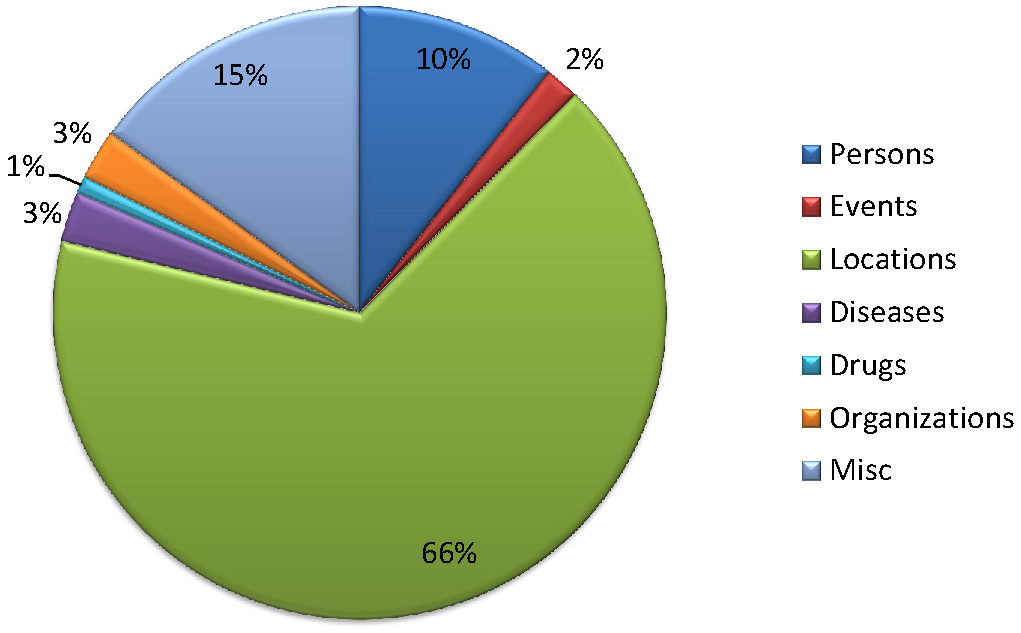
\includegraphics[width=0.5\textwidth]{img/specDistribution_cropped.pdf}

	\label{fig:specdistribution}
	\end{figure}
	\end{itemize}
	 
	

\end{frame}
%%%%%%%%%%%%%%%%%%%%%%%%%%%%%%%%%%%%%%%%%%%%%%%%%%%%%%%%%%%%%%%%%%%%%%%%%%%%%%%%%%%%%%%%%%%%%%%%%%%%%%%%%%%%%%%%%%%%%%%%%%%%%%%%%%%%%%%%%
\section{Results}
\begin{frame}
	\frametitle{First Experiments Set Results}
	\begin{itemize}
	  \item Detecting right specification average is 81\%
	  \item Detecting right specifications in geo-spatial domain is 92\%
	  \item Detecting right specifications in persons domain is 58.3\%
	 \end{itemize}
	 \begin{figure}[htb]

	 \centering

		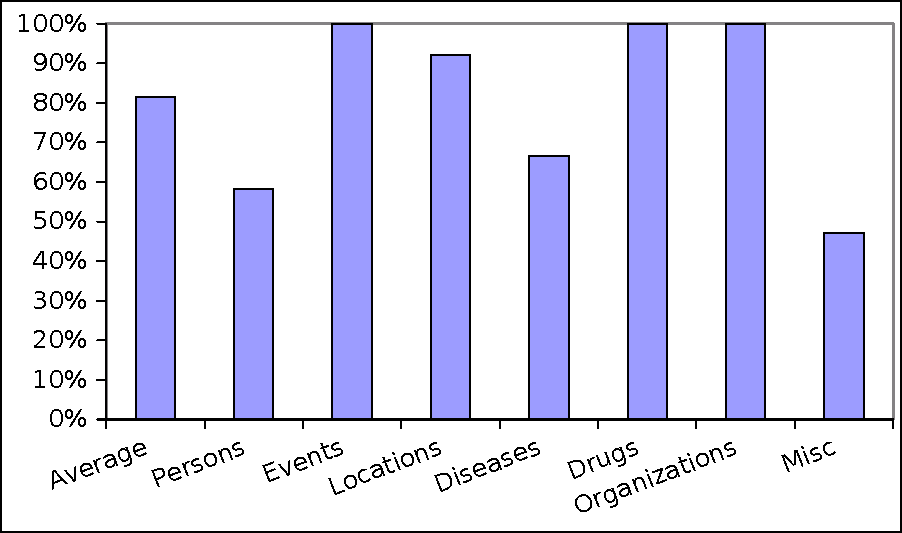
\includegraphics[width=0.5\textwidth]{img/mrr.pdf}

	\label{fig:specdistribution}
	\end{figure}

\end{frame}
\begin{frame}
	\frametitle{Second Experiments Set Results}
	In the second Experiments series, both source and target endpoints considered to be alive.\\
	 \begin{figure}[htb]

	\centering

		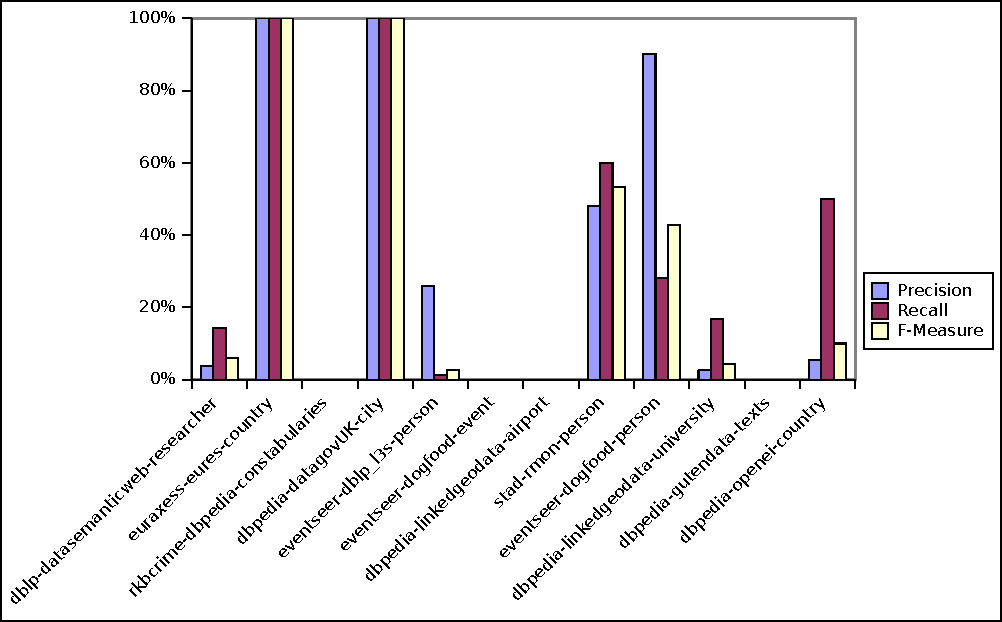
\includegraphics[width=0.5\textwidth]{img/uribasedprf.pdf}

	\label{fig:specdistribution}
	\end{figure}

\end{frame}
%%%%%%%%%%%%%%%%%%%%%%%%%%%%%%%%%%%%%%%%%%%%%%%%%%%%%%%%%%%%%%%%%%%%%%%%%%%%%%%%%%%%%%%%%%%%%%%%%%%%%%%%%%%%%%%%%%%%%%%%%%%%%%%%%%%%%%%%%
\section{Conclusion}

\begin{frame}[fragile]
	\frametitle{Conclusion}
\begin{itemize}
		  \item Detecting best similar specification with mean reciprocal rank larger than or equal 0.81
		  \item Transfer learning can not  replace the learning of link specification in itself
\end{itemize}
\end{frame}
%%%%%%%%%%%%%%%%%%%%%%%%%%%%%%%%%%%%%%%%%%%%%%%%%%%%%%%%%%%%%%%%%%%%%%%%%%%%%%%%%%%%%%%%%%%%%%%%%%%%%%%%%%%%%%%%%%%%%%%%%%%%%%%%%%%%%%%%
\section{Future Work}

\begin{frame}[fragile]
	\frametitle{Future Work}
\begin{itemize}
		  \item Combining other learning approaches of link specification to transfer learning
		  \item Using more sophisticated class and property similarity approaches 
\end{itemize}
\end{frame}
%%%%%%%%%%%%%%%%%%%%%%%%%%%%%%%%%%%%%%%%%%%%%%%%%%%%%%%%%%%%%%%%%%%%%%%%%%%%%%%%%%%%%%%%%%%%%%%%%%%%%%%%%%%%%%%%%%%%%%%%%%%%%%%%%%%%%%%%%
\section{Questions?}

\begin{frame}
	\frametitle{Questions}
\end{frame}
      ?
\end{document}
